% MATH 573 HW 3
% LUKE WUKMER

\documentclass[10pt]{article}

% note: some of these are extremely useful and i don't remember why :o
%\usepackage{savetrees} % disable custom geometry stuff if you do this
\usepackage{amsmath, amsthm, amssymb, amsfonts}
\usepackage{amsxtra, amscd, geometry, graphicx}
\usepackage{endnotes}
\usepackage{cancel}
\usepackage{bm} %allows fancy stuff like bold greek in math mode
\usepackage{alltt}
\usepackage{enumerate} %more/easier control over lists, also see enumitem
%\usepackage[all,cmtip]{xypic}
\usepackage{mathrsfs}
\usepackage{listings}
\usepackage{caption}
%\usepackage{subfigure}
%\usepackage{subcaption}
%\usepackage[pdftex]{hyperref}
%\usepackage[dvips,bookmarks,bookmarksopen,backref,colorlinks,linkcolor={blue},citecolor={blue},urlcolor={blue}](hyperref}


% change up the fonts (pick one only)
%\usepackage{times}%
\usepackage{helvet}%
%\usepackage{palatino}%
%\usepackage{bookman}%

% These are italic.
\theoremstyle{plain}
\newtheorem{thm}{Theorem}
\newtheorem*{thm*}{Theorem}
\newtheorem{prop}{Proposition}
\newtheorem*{prop*}{Proposition}
\newtheorem{conj}{Conjecture}
\newtheorem*{conj*}{Conjecture}
\newtheorem{lem}{Lemma}
  \makeatletter
  \@addtoreset{lem}{thm}
  \makeatother 
\newtheorem*{lem*}{Lemma}
\newtheorem{cor}{Corollary}
  \makeatletter
  \@addtoreset{cor}{thm}
  \makeatother 
\newtheorem*{cor*}{Corollary}

%\newtheorem{lem}[thm]{Lemma}
%\newtheorem{remark}[thm]{Remark}
%\newtheorem{cor}[thm]{Corollary}
%\newtheorem{prop}[thm]{Proposition}
%\newtheorem{conj}[thm]{Conjecture}

% These are normal (i.e. not italic).
\theoremstyle{definition}
\newtheorem*{ack*}{Acknowledgements}
\newtheorem*{app*}{Application}
\newtheorem*{apps*}{Applications}
\newtheorem{defn}{Definition}
\newtheorem*{defn*}{Definition}
\newtheorem{eg}{Example}
  \makeatletter
  \@addtoreset{eg}{thm}
  \makeatother 
\newtheorem*{eg*}{Example}
\newtheorem*{egs*}{Examples}
\newtheorem{ex}{Exercise}
\newtheorem*{ex*}{Exercise}
\newtheorem*{quest*}{Question}
\newtheorem{rem}{Remark}
\newtheorem*{rem*}{Remark}
\newtheorem{rems}{Remarks}
\newtheorem*{rems*}{Remarks}
\newtheorem{prob}{Problem}
\newtheorem*{prob*}{Problem}
\newtheorem*{soln*}{Solution}
\newtheorem{soln}{Solution}


% New Commands: Common Math Symbols
\providecommand{\R}{\mathbb{R}}%
\providecommand{\N}{\mathbb{N}}%
\providecommand{\Z}{{\mathbb{Z}}}%
\providecommand{\sph}{\mathbb{S}}%
\providecommand{\Q}{\mathbb{Q}}%
\providecommand{\C}{{\mathbb{C}}}%
\providecommand{\F}{\mathbb{F}}%
\providecommand{\quat}{\mathbb{H}}%

% haha, i originally forked this template from one provided by my abstract
% algebra TA (back in 2012 or something). probably don't need most of these,
% huh. 

% New Commands: Operators
\providecommand{\Gal}{\operatorname{Gal}}%
\providecommand{\GL}{\operatorname{GL}}%
\providecommand{\card}{\operatorname{card}}%
\providecommand{\coker}{\operatorname{coker}}%
\providecommand{\id}{\operatorname{id}}%
\providecommand{\im}{\operatorname{im}}%
\providecommand{\diam}{{\rm diam}}%
\providecommand{\aut}{\operatorname{Aut}}%
\providecommand{\inn}{\operatorname{Inn}}%
\providecommand{\out}{{\rm Out}}%
\providecommand{\End}{{\rm End}}%
\providecommand{\rad}{{\rm Rad}}%
\providecommand{\rk}{{\rm rank}}%
\providecommand{\ord}{{\rm ord}}%
\providecommand{\tor}{{\rm Tor}}%
\providecommand{\comp}{{\text{ $\scriptstyle \circ$ }}}%
\providecommand{\cl}[1]{\overline{#1}}%
\providecommand{\tr}{{\sf trace}}%

\renewcommand{\tilde}[1]{\widetilde{#1}}%
\numberwithin{equation}{section}

% i like the squiggly ones more. add as needed

\renewcommand{\Psi}{\varPsi}

\newcommand*\rfrac[2]{{}^{#1}\!/_{#2}}

% a very fancy dot product \ip{f}{g}
\newcommand\ip[2]{ \left\langle {#1} , {#2} \right\rangle }

% "s.t." for math mode
\providecommand{\st}{\text{ s.t. }}

% \norm{f} and such, super useful
\newcommand{\norm}[1]{\left\lVert#1\right\rVert}

% determinant
%\newcommand{\det}[1]{\textsf{det}\left(#1\right)}

% jacobian
\providecommand{\J}{\textsf{J}}

% this makes the spacing between lines of font a little bigger
%\newcommand{\spacing}[1]{\renewcommand{\baselinestretch}{#1}\large\normalsize}
%\spacing{1.2}

\newcommand*\mcol[1]{\overset{\big\uparrow}{\underset{\big\downarrow}{#1}}}

% Makes the margin size a little smaller, i gots stuff to say
%\geometry{letterpaper,margin=1.2}
% END PREAMBLE %%%%%%%%%%%%%%%%%%%%%%%%%
%%%%%%%%%%%%%%%%%%%%%%%%%%%%%%%%%%%%%%%%


\begin{document}

\title{Math 573 HW\textsuperscript{\#}3}
\author{Luke Wukmer}
\date{Fall 2015}
\maketitle \thispagestyle{empty} % remove the page number from the first page

%%% PROBLEM 1
\begin{prob}
    Least squares polynomial of degree $\leq n$, $p(x) = \sum_{k=0}^n a_k x^k$
    with $m>n$ data points given by

    \[      \mathbb{X}^T\mathbb{X}\, \bm{a} = \mathbb{X}^T \bm{y}
    \]
    where \[
            \mathbb{X} := \begin{bmatrix}
                \uparrow & \uparrow & \uparrow &    & \uparrow \\
            1       & x_i & (x_i)^2 & \cdots & (x_i)^n      \\\
            \downarrow & \downarrow & \downarrow &  & \downarrow 
            \end{bmatrix}
\]

\begin{enumerate}[\bfseries(a)]
\item $n=2$: 
\item $n=3$:
    Setting $\frac{\partial E_2(a_0, \ldots , a_3)}{\partial a_i} = 0$ for each $i$
    results in the system
\[
\begin{bmatrix}
    4          & \sum (x_i)   & \sum x_i^2 & \sum x_i^3 \\
    \sum x_i   & \sum (x_i)^2 & \sum x_i^3 & \sum x_i^4 \\
    \sum x_i^2 & \sum (x_i)^3 & \sum x_i^4 & \sum x_i^5 \\
    \sum x_i^3 & \sum (x_i)^4 & \sum x_i^5 & \sum x_i^6 \\
\end{bmatrix}
\begin{bmatrix} a_0 \\ a_1 \\ a_2 \\ a_3 \end{bmatrix}
=
\begin{bmatrix} \sum y_i \\ \sum y_i x_i \\ \sum y_i x_i^2 \\ \sum y_i x_i^3 \end{bmatrix}
\]
Substituting in the values from Table 1, we have
\[
\begin{pmatrix}
4.      &   4.9     &   6.15    &   7.903   \\
4.9     &   6.15    &   7.903   &  10.3827  \\
6.15    &   7.903   &  10.3827  &  13.91719 \\
7.903   &  10.3827  &  13.91719 &  18.988995
\end{pmatrix}
\begin{bmatrix} a_0 \\ a_1 \\ a_2 \\ a_3 \end{bmatrix}
= \begin{pmatrix} 8.46    \\ 10.544   \\ 13.459   \\ 17.57288 \end{pmatrix}
\]
whose solution is
$\bm{a} = \begin{bmatrix} 1.6575 & -1.38416667 & 2.15 & -0.58333333 \end{bmatrix}^T$. Thus
the least-squares polynomial of degree 3 is
\[
        y = p_3(x) = 1.6575  - 1.38416667 x + 2.15 x^2  - 0.58333333 x^3
\]

\item   $y= bx^a$ \textit{form}:
    Solving the equations $\frac{\partial E_2}{\partial a} , \frac{\partial E_2}{\partial b}$
    results in a nasty system of nonlinear equations, so we search for the
    linearized form of our target equation.
\end{enumerate}
\end{prob}
%%% PROBLEM 2
\begin{prob}
    A cardinal spline is a sequence of individual curves joined to form a
    larger curve. The spline is specified by an array of points and a tension
    parameter, $c$. A cardinal spline passes smoothly through each point in the
    array; there are no sharp corners and no abrupt changes in the tightness
    of the curve. A cardinal spline (often used to make a polygon) uses an
    alternative formula for calculating the tangents at each interval
    (compared to Hermite curves). In particular, 
    \[
            m_k = \frac{1}{2}(1-c)\left(P_{k+1} - P_{k-1}\right)
        \]
    is used to calculate the tangent at $P_k$, where $c$ is between 0 and 1.
    Find the blending functions of the cardinal splines.
\end{prob}

\begin{soln*}
    We formulate a sequence of cardinal splines for some control points
    $\{P_k\}_{k=1}^{N} \subset \R^3$ and
    a fixed tension parameter $c \in {[0,1)}$. For $ 1 < k < N-1$,
        our goal is to create a spline $\bm{p}_k(t)$ satisfying the following: 
    \begin{gather*}
    \bm{p}_k: {[0,1]} \rightarrow \R^3 \quad \st \quad
    \bm{p}_k(0) = P_k , \; \bm{p}_k(1) = P_{k+1} , \\
    \bm{p}'(0) = m_k = \frac{1}{2}(1-c)\left(P_{k+1} - P_{k-1}\right) \quad
    \bm{p}'(1) = m_{k+1} = \frac{1}{2}(1-c)\left(P_{k+2} - P_{k}\right) 
    \end{gather*}
    Thus, each $\bm{p}_k(t)$ is specified by the geometry
    $G_C := \begin{bmatrix} P_{k-1} & P_k & P_{k+1} & P_{k+2} \end{bmatrix}^T$.
    Using the conditions above, we can readily convert between the geometries
    of Hermite/cardinal via
    \[
            \underbrace{\begin{bmatrix}
                0 & 1 & 0 & 0 \\
                0 & 0 & 1 & 0 \\
                -\frac{1}{2}(1-c) & 0 & \frac{1}{2}(1-c) & 0 \\
                0 & -\frac{1}{2}(1-c) & 0 & \frac{1}{2}(1-c)
                \end{bmatrix}}_{M_{HC}}
            \underbrace{
            \begin{bmatrix}
                P_{k-1} \\ P_k \\ P_{k+1} \\ P_{k+2}
        \end{bmatrix}}_{G_C}
            =
            \underbrace{
            \begin{bmatrix}
                \bm{p}(0) \\ \bm{p}(1) \\ \bm{p}'(0) \\ \bm{p}'(1)
        \end{bmatrix}}_{G_H}
        \]
    We substitute $G_H = M_{HC} G_C$ directly into the solution for Hermite curves:
    \[
            \bm{p}_k(t) = \bm{t}^T C = \bm{t}^T M_H G_H = \bm{t}^T M_H (M_{HC} G_C )
                        = \bm{t}^T M_C G_C 
                        = (M_C^T \bm{t})^T \cdot G_C
        \]
        where we define $M_C := M_H M_{HC}$. Solving,
    \begin{align*}
            M_C := M_H M_{HC}
            &= \begin{bmatrix}
                2 & {-2} & 1 & 1 \\
                {-3} & 3 & {-2} & -1 \\
                0 & 0 & 1 & 0 \\
                1 & 0 & 0 & 0 \end{bmatrix}
            \begin{bmatrix}
                0 & 1 & 0 & 0 \\
                0 & 0 & 1 & 0 \\
                -\frac{1}{2}(1-c) & 0 & \frac{1}{2}(1-c) & 0 \\
                0 & -\frac{1}{2}(1-c) & 0 & \frac{1}{2}(1-c)
            \end{bmatrix} \\
            &= 
            \frac{1}{2} \begin{bmatrix}
                (c-1)   & (c+3)     & -(c+3)    & -(c-1)    \\
                -2(c-1) & -(c+5)    & 2(c+2)    & (c-1)     \\
                (c-1)   & 0         & -(c-1)    & 0         \\
                0       & 2         & 0         & 2
            \end{bmatrix}
    \end{align*}
    
    As with Hermite curves, we can define the blending functions
    $\bm{b}(t) = M_C^T \bm{t}$, with
    \begin{align*}
    \bm{b}(t) = M_C^T \bm{t}
              = 
            \frac{1}{2} \begin{bmatrix}
                (c-1)   & -2(c-1)   & (c-1)     & 0         \\
                (c+3)   & -(c+5)    & 0         & 2         \\
                -(c+3)  & 2(c+2)    & -(c-1)    & 0         \\
                -(c-1)  & (c-1)     & 0         & 2
            \end{bmatrix}
    \begin{bmatrix} t^3 \\ t^2 \\ t \\ 1 \end{bmatrix} \\
          =  \frac{1}{2} \begin{bmatrix}
              (c-1)   t^3 -2(c-1) t^2  + (c-1)  t \\ 
              (c+3)   t^3 -(c+5)  t^2    +     t   + 2         \\
              -(c+3)  t^3 + 2(c+2)  t^2  -(c-1) t  \\ 
              -(c-1)  t^3 + (c-1)   t^2  + 2
            \end{bmatrix}
            \begin{matrix}
                =: b_1(t) \\
                =: b_2(t) \\
                =: b_3(t) \\
                =: b_4(t) 
            \end{matrix}
    \end{align*}

We plot these blending functions for several values of $c$ below.
\begin{figure}[h]
    \centering
    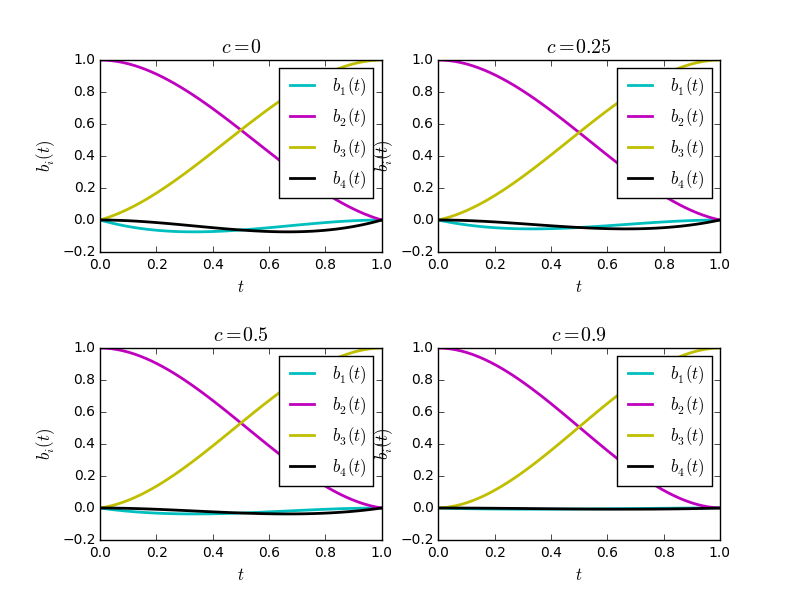
\includegraphics[width=1\textwidth]{cardinals}
    \caption{Graphing the blending functions of the cardinal spline for several values of $c$.}
\end{figure}
\end{soln*}
%%% PROBLEM 3
\begin{prob}
    Least squares line
\end{prob}
%%% PROBLEM 4
\begin{prob}
    B-splines.
    \begin{figure}[h]
        \centering
        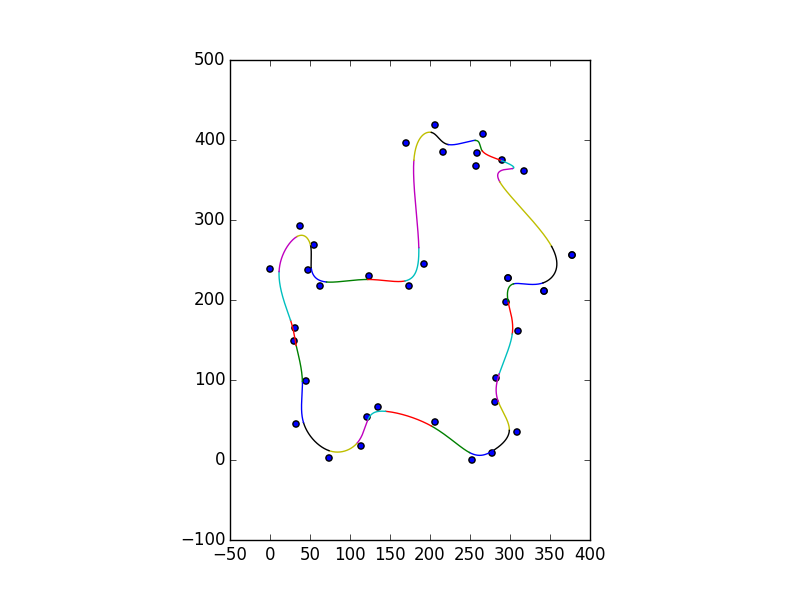
\includegraphics[width=\textwidth]{doggy_splines}
        %\caption{B-spline fitting of the data in Table 3}
    \end{figure}
\end{prob}
%%%%%%%%%%%%%%%%%%%%%%%%%%%%%%%%%%%%%%%%%%%%%%%%%%%%%%%%%%%%%%%%%%%%%%%%%%%%%%
\end{document}
